\documentclass[12pt,]{article}
\usepackage{lmodern}
\usepackage{amssymb,amsmath}
\usepackage{ifxetex,ifluatex}
\usepackage{fixltx2e} % provides \textsubscript
\ifnum 0\ifxetex 1\fi\ifluatex 1\fi=0 % if pdftex
  \usepackage[T1]{fontenc}
  \usepackage[utf8]{inputenc}
\else % if luatex or xelatex
  \ifxetex
    \usepackage{mathspec}
  \else
    \usepackage{fontspec}
  \fi
  \defaultfontfeatures{Ligatures=TeX,Scale=MatchLowercase}
    \setmainfont[]{Times New Roman}
\fi
% use upquote if available, for straight quotes in verbatim environments
\IfFileExists{upquote.sty}{\usepackage{upquote}}{}
% use microtype if available
\IfFileExists{microtype.sty}{%
\usepackage{microtype}
\UseMicrotypeSet[protrusion]{basicmath} % disable protrusion for tt fonts
}{}
\usepackage[margin=2.54cm]{geometry}
\usepackage{hyperref}
\hypersetup{unicode=true,
            pdftitle={Changes in Land Use between 1990 and 2014},
            pdfauthor={Rebecca Marx},
            pdfborder={0 0 0},
            breaklinks=true}
\urlstyle{same}  % don't use monospace font for urls
\usepackage{color}
\usepackage{fancyvrb}
\newcommand{\VerbBar}{|}
\newcommand{\VERB}{\Verb[commandchars=\\\{\}]}
\DefineVerbatimEnvironment{Highlighting}{Verbatim}{commandchars=\\\{\}}
% Add ',fontsize=\small' for more characters per line
\usepackage{framed}
\definecolor{shadecolor}{RGB}{248,248,248}
\newenvironment{Shaded}{\begin{snugshade}}{\end{snugshade}}
\newcommand{\KeywordTok}[1]{\textcolor[rgb]{0.13,0.29,0.53}{\textbf{#1}}}
\newcommand{\DataTypeTok}[1]{\textcolor[rgb]{0.13,0.29,0.53}{#1}}
\newcommand{\DecValTok}[1]{\textcolor[rgb]{0.00,0.00,0.81}{#1}}
\newcommand{\BaseNTok}[1]{\textcolor[rgb]{0.00,0.00,0.81}{#1}}
\newcommand{\FloatTok}[1]{\textcolor[rgb]{0.00,0.00,0.81}{#1}}
\newcommand{\ConstantTok}[1]{\textcolor[rgb]{0.00,0.00,0.00}{#1}}
\newcommand{\CharTok}[1]{\textcolor[rgb]{0.31,0.60,0.02}{#1}}
\newcommand{\SpecialCharTok}[1]{\textcolor[rgb]{0.00,0.00,0.00}{#1}}
\newcommand{\StringTok}[1]{\textcolor[rgb]{0.31,0.60,0.02}{#1}}
\newcommand{\VerbatimStringTok}[1]{\textcolor[rgb]{0.31,0.60,0.02}{#1}}
\newcommand{\SpecialStringTok}[1]{\textcolor[rgb]{0.31,0.60,0.02}{#1}}
\newcommand{\ImportTok}[1]{#1}
\newcommand{\CommentTok}[1]{\textcolor[rgb]{0.56,0.35,0.01}{\textit{#1}}}
\newcommand{\DocumentationTok}[1]{\textcolor[rgb]{0.56,0.35,0.01}{\textbf{\textit{#1}}}}
\newcommand{\AnnotationTok}[1]{\textcolor[rgb]{0.56,0.35,0.01}{\textbf{\textit{#1}}}}
\newcommand{\CommentVarTok}[1]{\textcolor[rgb]{0.56,0.35,0.01}{\textbf{\textit{#1}}}}
\newcommand{\OtherTok}[1]{\textcolor[rgb]{0.56,0.35,0.01}{#1}}
\newcommand{\FunctionTok}[1]{\textcolor[rgb]{0.00,0.00,0.00}{#1}}
\newcommand{\VariableTok}[1]{\textcolor[rgb]{0.00,0.00,0.00}{#1}}
\newcommand{\ControlFlowTok}[1]{\textcolor[rgb]{0.13,0.29,0.53}{\textbf{#1}}}
\newcommand{\OperatorTok}[1]{\textcolor[rgb]{0.81,0.36,0.00}{\textbf{#1}}}
\newcommand{\BuiltInTok}[1]{#1}
\newcommand{\ExtensionTok}[1]{#1}
\newcommand{\PreprocessorTok}[1]{\textcolor[rgb]{0.56,0.35,0.01}{\textit{#1}}}
\newcommand{\AttributeTok}[1]{\textcolor[rgb]{0.77,0.63,0.00}{#1}}
\newcommand{\RegionMarkerTok}[1]{#1}
\newcommand{\InformationTok}[1]{\textcolor[rgb]{0.56,0.35,0.01}{\textbf{\textit{#1}}}}
\newcommand{\WarningTok}[1]{\textcolor[rgb]{0.56,0.35,0.01}{\textbf{\textit{#1}}}}
\newcommand{\AlertTok}[1]{\textcolor[rgb]{0.94,0.16,0.16}{#1}}
\newcommand{\ErrorTok}[1]{\textcolor[rgb]{0.64,0.00,0.00}{\textbf{#1}}}
\newcommand{\NormalTok}[1]{#1}
\usepackage{graphicx,grffile}
\makeatletter
\def\maxwidth{\ifdim\Gin@nat@width>\linewidth\linewidth\else\Gin@nat@width\fi}
\def\maxheight{\ifdim\Gin@nat@height>\textheight\textheight\else\Gin@nat@height\fi}
\makeatother
% Scale images if necessary, so that they will not overflow the page
% margins by default, and it is still possible to overwrite the defaults
% using explicit options in \includegraphics[width, height, ...]{}
\setkeys{Gin}{width=\maxwidth,height=\maxheight,keepaspectratio}
\IfFileExists{parskip.sty}{%
\usepackage{parskip}
}{% else
\setlength{\parindent}{0pt}
\setlength{\parskip}{6pt plus 2pt minus 1pt}
}
\setlength{\emergencystretch}{3em}  % prevent overfull lines
\providecommand{\tightlist}{%
  \setlength{\itemsep}{0pt}\setlength{\parskip}{0pt}}
\setcounter{secnumdepth}{5}
% Redefines (sub)paragraphs to behave more like sections
\ifx\paragraph\undefined\else
\let\oldparagraph\paragraph
\renewcommand{\paragraph}[1]{\oldparagraph{#1}\mbox{}}
\fi
\ifx\subparagraph\undefined\else
\let\oldsubparagraph\subparagraph
\renewcommand{\subparagraph}[1]{\oldsubparagraph{#1}\mbox{}}
\fi

%%% Use protect on footnotes to avoid problems with footnotes in titles
\let\rmarkdownfootnote\footnote%
\def\footnote{\protect\rmarkdownfootnote}

%%% Change title format to be more compact
\usepackage{titling}

% Create subtitle command for use in maketitle
\providecommand{\subtitle}[1]{
  \posttitle{
    \begin{center}\large#1\end{center}
    }
}

\setlength{\droptitle}{-2em}

  \title{Changes in Land Use between 1990 and 2014}
    \pretitle{\vspace{\droptitle}\centering\huge}
  \posttitle{\par}
  \subtitle{\url{https://github.com/RsMarx/Ag_Forest_Data_Final-}}
  \author{Rebecca Marx}
    \preauthor{\centering\large\emph}
  \postauthor{\par}
    \date{}
    \predate{}\postdate{}
  

\begin{document}
\maketitle
\begin{abstract}
Experimental overview. This section should be no longer than 250 words.
\end{abstract}

\newpage

\tableofcontents  \newpage
\listoftables  \newpage
\listoffigures  \newpage

\textless{}Note: set up autoreferencing for figures and tables in your
document\textgreater{}

\section{Research Question and
Rationale}\label{research-question-and-rationale}

As the global population continues to grow and require more food and
fuel resources, deforestation trends are expected to accelerate.
Deforestation can be problematic as forests provide ecosystem services
such as carbon storage, nutrient cycling, water filtration, and wildlife
habitat. Agriculture is one of the most commonly sited drivers of
deforestation, in addition to being a source of emissions. Given that
forest and agriculture can be contending land uses, this research
examines the relationship between agriculture and forest as land uses
and, more broadly, explores the causes and impacts of changes in land
use.

This research looks at the trends and tradeoffs in land use across
countries from 1990 -- 2014. Primary questions include:

\begin{itemize}
\tightlist
\item
  Is there a relationship between the percentage of land area dedicated
  to forest versus agricultural in countries?
\item
  Is there a relationship between land uses (agriculture or forest) and
  levels of CO2, methane, and NO3 emissions?
\item
  Is there a relationship between access to electricity or renewable
  electricity output and the percentage of land dedicated to forestry
  versus agriculture?
\end{itemize}

The research utilizes a data set from the World Bank that has 135
environment-related variables for 264 countries. I have narrowed the
environment variable down to 9 that are relevant to land use. Although
the full data set dates back to 1960, I have limited to the time scope
of the analysis to between 1990 and 2014 because those are the dates for
which forest cover data is available.

\newpage

\section{Dataset Information}\label{dataset-information}

\newpage

\section{Exploratory Data Analysis and
Wrangling}\label{exploratory-data-analysis-and-wrangling}

\begin{Shaded}
\begin{Highlighting}[]
\NormalTok{World_Bank_Master <-}\KeywordTok{read.csv}\NormalTok{(}\StringTok{"../Raw/WorldBank_Raw2_4.8.19.csv"}\NormalTok{)}

\CommentTok{#Data Subset}
\NormalTok{World_Bank_Filter <-}\StringTok{ }\KeywordTok{filter}\NormalTok{(World_Bank_Master, Indicator.Name }\OperatorTok{==}\StringTok{ "Forest area (% of land area)"} \OperatorTok{|}\StringTok{ }\NormalTok{Indicator.Name }\OperatorTok{==}\StringTok{ "Agricultural land (% of land area)"} \OperatorTok{|}\StringTok{ }\NormalTok{Indicator.Name }\OperatorTok{==}\StringTok{ "Arable land (% of land area)"} \OperatorTok{|}\StringTok{ }\NormalTok{Indicator.Name }\OperatorTok{==}\StringTok{ "Access to electricity (% of population)"} \OperatorTok{|}\StringTok{ }\NormalTok{Indicator.Name }\OperatorTok{==}\StringTok{ "Renewable electricity output (% of total electricity output)"} \OperatorTok{|}\StringTok{ }\NormalTok{Indicator.Name }\OperatorTok{==}\StringTok{ "CO2 emissions (kt)"} \OperatorTok{|}\StringTok{ }\NormalTok{Indicator.Name }\OperatorTok{==}\StringTok{ "Agricultural nitrous oxide emissions (thousand metric tons of CO2 equivalent)"} \OperatorTok{|}\StringTok{ }\NormalTok{Indicator.Name }\OperatorTok{==}\StringTok{ "Agricultural methane emissions (thousand metric tons of CO2 equivalent)"} \OperatorTok{|}\StringTok{ }\NormalTok{Indicator.Name }\OperatorTok{==}\StringTok{ "Aquaculture production (metric tons)"}\NormalTok{)}

\NormalTok{WorldBank_Gather <-}\StringTok{ }\KeywordTok{gather}\NormalTok{(World_Bank_Filter, }\StringTok{"Year"}\NormalTok{, }\StringTok{"Level"}\NormalTok{, X1960}\OperatorTok{:}\NormalTok{X2018)}

\NormalTok{WorldBank_Gather <-}\StringTok{ }\KeywordTok{select}\NormalTok{(WorldBank_Gather, }\OperatorTok{-}\NormalTok{Indicator.Code)}

\NormalTok{WorldBank_Spread <-}\StringTok{  }\KeywordTok{spread}\NormalTok{(WorldBank_Gather, Indicator.Name, Level)}

\CommentTok{#Format as character }
\NormalTok{WorldBank_Spread}\OperatorTok{$}\NormalTok{Year <-}\StringTok{ }\KeywordTok{as.character}\NormalTok{(WorldBank_Spread}\OperatorTok{$}\NormalTok{Year)}

\CommentTok{#create string}
\NormalTok{WB_String <-}\StringTok{ }\KeywordTok{substr}\NormalTok{(WorldBank_Spread}\OperatorTok{$}\NormalTok{Year, }\DecValTok{2}\NormalTok{, }\DecValTok{5}\NormalTok{)}

\CommentTok{#Get rid of X in date}
\NormalTok{WorldBank_Spread}\OperatorTok{$}\NormalTok{Year =}\StringTok{ }\NormalTok{WB_String}

\CommentTok{#Format as date}
\CommentTok{#WB_Fixed$Year <- as.Date(WB_Fixed$Year)}
\NormalTok{WorldBank_Spread}\OperatorTok{$}\NormalTok{Year <-}\StringTok{ }\KeywordTok{as.Date}\NormalTok{(WorldBank_Spread}\OperatorTok{$}\NormalTok{Year, }\DataTypeTok{format =} \StringTok{"%Y"}\NormalTok{) }\CommentTok{#can I get it to show only the year? }

\KeywordTok{class}\NormalTok{(WorldBank_Spread}\OperatorTok{$}\NormalTok{Year)}
\end{Highlighting}
\end{Shaded}

\begin{verbatim}
## [1] "Date"
\end{verbatim}

\begin{Shaded}
\begin{Highlighting}[]
\CommentTok{#Change column names }
\KeywordTok{names}\NormalTok{(WorldBank_Spread) <-}\StringTok{ }\KeywordTok{c}\NormalTok{(}\StringTok{"Country"}\NormalTok{, }\StringTok{"Indicator.Code"}\NormalTok{, }\StringTok{"Year"}\NormalTok{, }\StringTok{"ElectricityAccess"}\NormalTok{, }\StringTok{"Agriculture"}\NormalTok{, }\StringTok{"Ag.Methane"}\NormalTok{, }\StringTok{"Ag.NO2"}\NormalTok{, }\StringTok{"Aquaculture"}\NormalTok{, }\StringTok{"ArableLand"}\NormalTok{, }\StringTok{"CO2Emissions"}\NormalTok{, }\StringTok{"Forest"}\NormalTok{, }\StringTok{"RenewableElectricity"}\NormalTok{)}

\CommentTok{#Save processed file }
\CommentTok{#write.csv(WorldBank_Spread, row.names = FALSE, file = "../Processed/WorldBank_Processed.csv")}
   
\NormalTok{Five_Countries <-}\StringTok{ }\KeywordTok{filter}\NormalTok{(WorldBank_Spread, Country }\OperatorTok{==}\StringTok{ "Brazil"} \OperatorTok{|}\StringTok{ }\NormalTok{Country }\OperatorTok{==}\StringTok{ "Kenya"} \OperatorTok{|}\StringTok{ }\NormalTok{Country }\OperatorTok{==}\StringTok{ "Spain"} \OperatorTok{|}\StringTok{ }\NormalTok{Country }\OperatorTok{==}\StringTok{ "Indonesia"} \OperatorTok{|}\StringTok{ }\NormalTok{Country }\OperatorTok{==}\StringTok{ "Canada"}\NormalTok{)}

\NormalTok{WB_Spread <-}\StringTok{ }\NormalTok{WorldBank_Spread }\OperatorTok
\StringTok{  }\NormalTok{na.exclude}

\NormalTok{WB_Brazil <-}\StringTok{ }\KeywordTok{filter}\NormalTok{(WB_Spread, Country }\OperatorTok{==}\StringTok{ "Brazil"}\NormalTok{)}
\end{Highlighting}
\end{Shaded}

\begin{verbatim}

<Include R chunks for 5+ lines of summary code (display code and output), 3+ exploratory graphs (display graphs only), and any wrangling you do to your dataset(s).> 

\end{verbatim}

\begin{Shaded}
\begin{Highlighting}[]
\CommentTok{#5+ lines of summary }

\KeywordTok{colnames}\NormalTok{(WorldBank_Spread)}
\end{Highlighting}
\end{Shaded}

\begin{verbatim}
##  [1] "Country"              "Indicator.Code"       "Year"                
##  [4] "ElectricityAccess"    "Agriculture"          "Ag.Methane"          
##  [7] "Ag.NO2"               "Aquaculture"          "ArableLand"          
## [10] "CO2Emissions"         "Forest"               "RenewableElectricity"
\end{verbatim}

\begin{Shaded}
\begin{Highlighting}[]
\KeywordTok{dim}\NormalTok{(WorldBank_Spread)}
\end{Highlighting}
\end{Shaded}

\begin{verbatim}
## [1] 15576    12
\end{verbatim}

\begin{Shaded}
\begin{Highlighting}[]
\KeywordTok{head}\NormalTok{(WorldBank_Spread)}
\end{Highlighting}
\end{Shaded}

\begin{verbatim}
##       Country Indicator.Code       Year ElectricityAccess Agriculture
## 1 Afghanistan            AFG 1960-04-15                NA          NA
## 2 Afghanistan            AFG 1961-04-15                NA    57.74592
## 3 Afghanistan            AFG 1962-04-15                NA    57.83782
## 4 Afghanistan            AFG 1963-04-15                NA    57.91441
## 5 Afghanistan            AFG 1964-04-15                NA    58.01091
## 6 Afghanistan            AFG 1965-04-15                NA    58.01397
##   Ag.Methane Ag.NO2 Aquaculture ArableLand CO2Emissions Forest
## 1         NA     NA          NA         NA      414.371     NA
## 2         NA     NA          NA   11.71767      491.378     NA
## 3         NA     NA          NA   11.79426      689.396     NA
## 4         NA     NA          NA   11.87085      707.731     NA
## 5         NA     NA          NA   11.94743      839.743     NA
## 6         NA     NA          NA   11.94743     1008.425     NA
##   RenewableElectricity
## 1                   NA
## 2                   NA
## 3                   NA
## 4                   NA
## 5                   NA
## 6                   NA
\end{verbatim}

\begin{Shaded}
\begin{Highlighting}[]
\KeywordTok{summary}\NormalTok{(WorldBank_Spread)}
\end{Highlighting}
\end{Shaded}

\begin{verbatim}
##            Country      Indicator.Code       Year           
##  Afghanistan   :   59   ABW    :   59   Min.   :1960-04-15  
##  Albania       :   59   AFG    :   59   1st Qu.:1974-04-15  
##  Algeria       :   59   AGO    :   59   Median :1989-04-15  
##  American Samoa:   59   ALB    :   59   Mean   :1989-04-14  
##  Andorra       :   59   AND    :   59   3rd Qu.:2004-04-15  
##  Angola        :   59   ARB    :   59   Max.   :2018-04-15  
##  (Other)       :15222   (Other):15222                       
##  ElectricityAccess  Agriculture        Ag.Methane          Ag.NO2         
##  Min.   :  0.00    Min.   : 0.2628   Min.   :      0   Min.   :      0.0  
##  1st Qu.: 53.11    1st Qu.:20.5547   1st Qu.:    120   1st Qu.:     86.9  
##  Median : 93.94    Median :37.3659   Median :   3300   Median :   2302.9  
##  Mean   : 75.04    Mean   :37.0790   Mean   : 117609   Mean   :  63590.8  
##  3rd Qu.:100.00    3rd Qu.:52.3930   3rd Qu.:  24198   3rd Qu.:  15076.6  
##  Max.   :100.00    Max.   :93.4407   Max.   :3464398   Max.   :2242932.7  
##  NA's   :8618      NA's   :2521      NA's   :5056      NA's   :5056       
##   Aquaculture          ArableLand       CO2Emissions     
##  Min.   :        0   Min.   : 0.0012   Min.   :     -81  
##  1st Qu.:       68   1st Qu.: 3.5315   1st Qu.:     964  
##  Median :     3758   Median : 9.5558   Median :   11463  
##  Mean   :  1601961   Mean   :13.1413   Mean   :  736069  
##  3rd Qu.:    95447   3rd Qu.:17.5690   3rd Qu.:  143107  
##  Max.   :106004184   Max.   :73.3886   Max.   :36138285  
##  NA's   :4696        NA's   :2658      NA's   :3321      
##      Forest         RenewableElectricity
##  Min.   :    0.00   Min.   :  0.000     
##  1st Qu.:   12.50   1st Qu.:  0.465     
##  Median :   31.18   Median : 16.961     
##  Mean   :   42.70   Mean   : 28.211     
##  3rd Qu.:   46.96   3rd Qu.: 49.255     
##  Max.   :16735.00   Max.   :100.000     
##  NA's   :8717       NA's   :8738
\end{verbatim}

\begin{Shaded}
\begin{Highlighting}[]
\KeywordTok{summary}\NormalTok{(WorldBank_Spread}\OperatorTok{$}\NormalTok{Agriculture)}
\end{Highlighting}
\end{Shaded}

\begin{verbatim}
##    Min. 1st Qu.  Median    Mean 3rd Qu.    Max.    NA's 
##  0.2628 20.5547 37.3659 37.0790 52.3930 93.4407    2521
\end{verbatim}

\begin{Shaded}
\begin{Highlighting}[]
\KeywordTok{summary}\NormalTok{(WorldBank_Spread}\OperatorTok{$}\NormalTok{Forest)}
\end{Highlighting}
\end{Shaded}

\begin{verbatim}
##     Min.  1st Qu.   Median     Mean  3rd Qu.     Max.     NA's 
##     0.00    12.50    31.18    42.70    46.96 16735.00     8717
\end{verbatim}

\begin{Shaded}
\begin{Highlighting}[]
\KeywordTok{summary}\NormalTok{(WorldBank_Spread}\OperatorTok{$}\NormalTok{RenewableElectricty)}
\end{Highlighting}
\end{Shaded}

\begin{verbatim}
## Length  Class   Mode 
##      0   NULL   NULL
\end{verbatim}

\begin{Shaded}
\begin{Highlighting}[]
\KeywordTok{summary}\NormalTok{(WB_Spread}\OperatorTok{$}\NormalTok{Ag.Methane)}
\end{Highlighting}
\end{Shaded}

\begin{verbatim}
##    Min. 1st Qu.  Median    Mean 3rd Qu.    Max. 
##       0    1258    6596  155800   53060 3464398
\end{verbatim}

\begin{verbatim}
## Warning: Removed 8897 rows containing missing values (geom_point).
\end{verbatim}

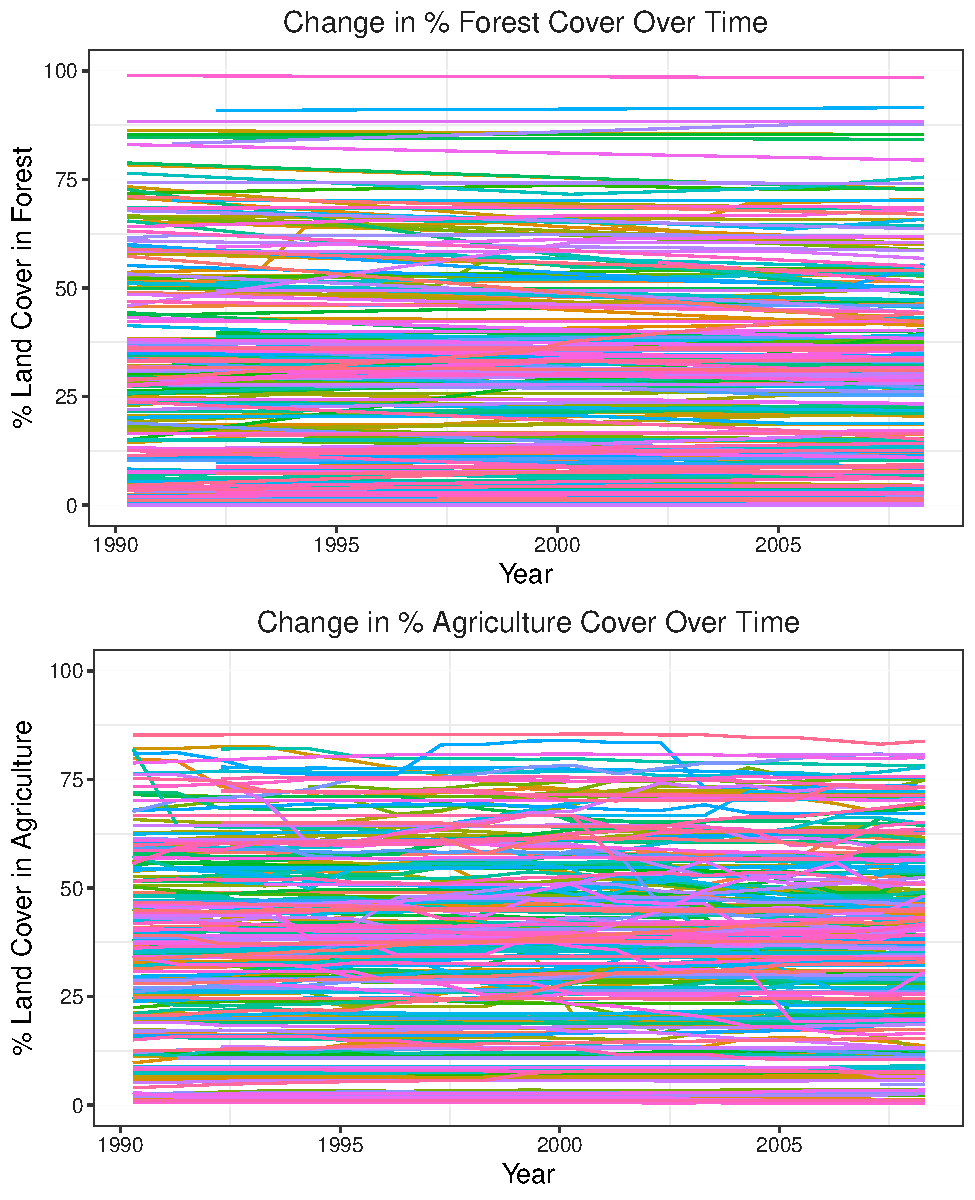
\includegraphics{Marx_ENV872_Project_files/figure-latex/unnamed-chunk-3-1.pdf}

\begin{verbatim}
## Warning: Removed 33 rows containing missing values (geom_path).
\end{verbatim}

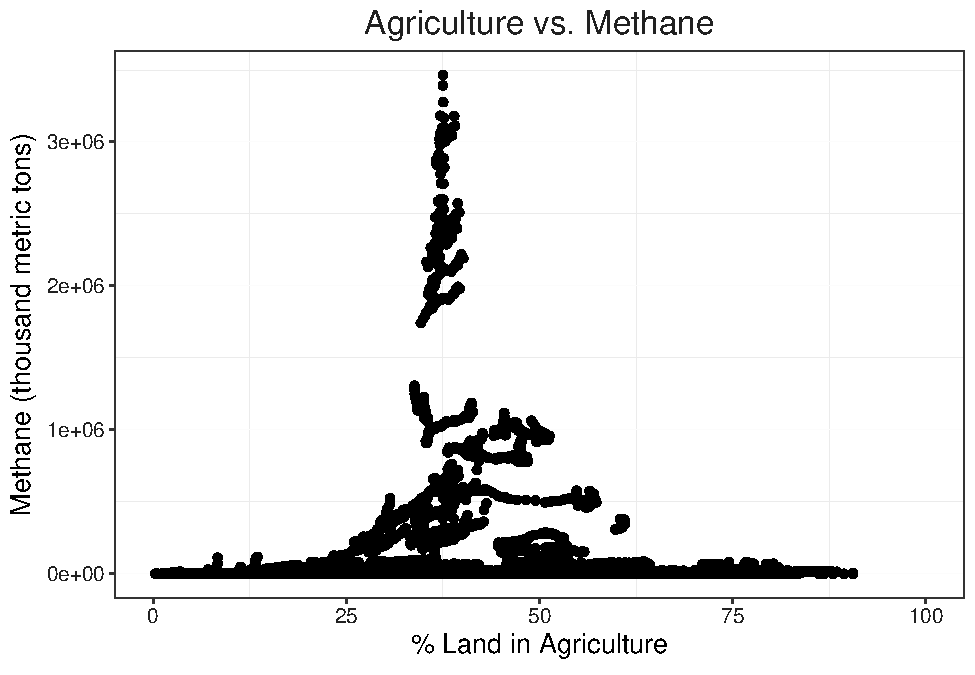
\includegraphics{Marx_ENV872_Project_files/figure-latex/unnamed-chunk-4-1.pdf}

\begin{verbatim}
## Warning: Removed 6297 rows containing missing values (geom_point).
\end{verbatim}

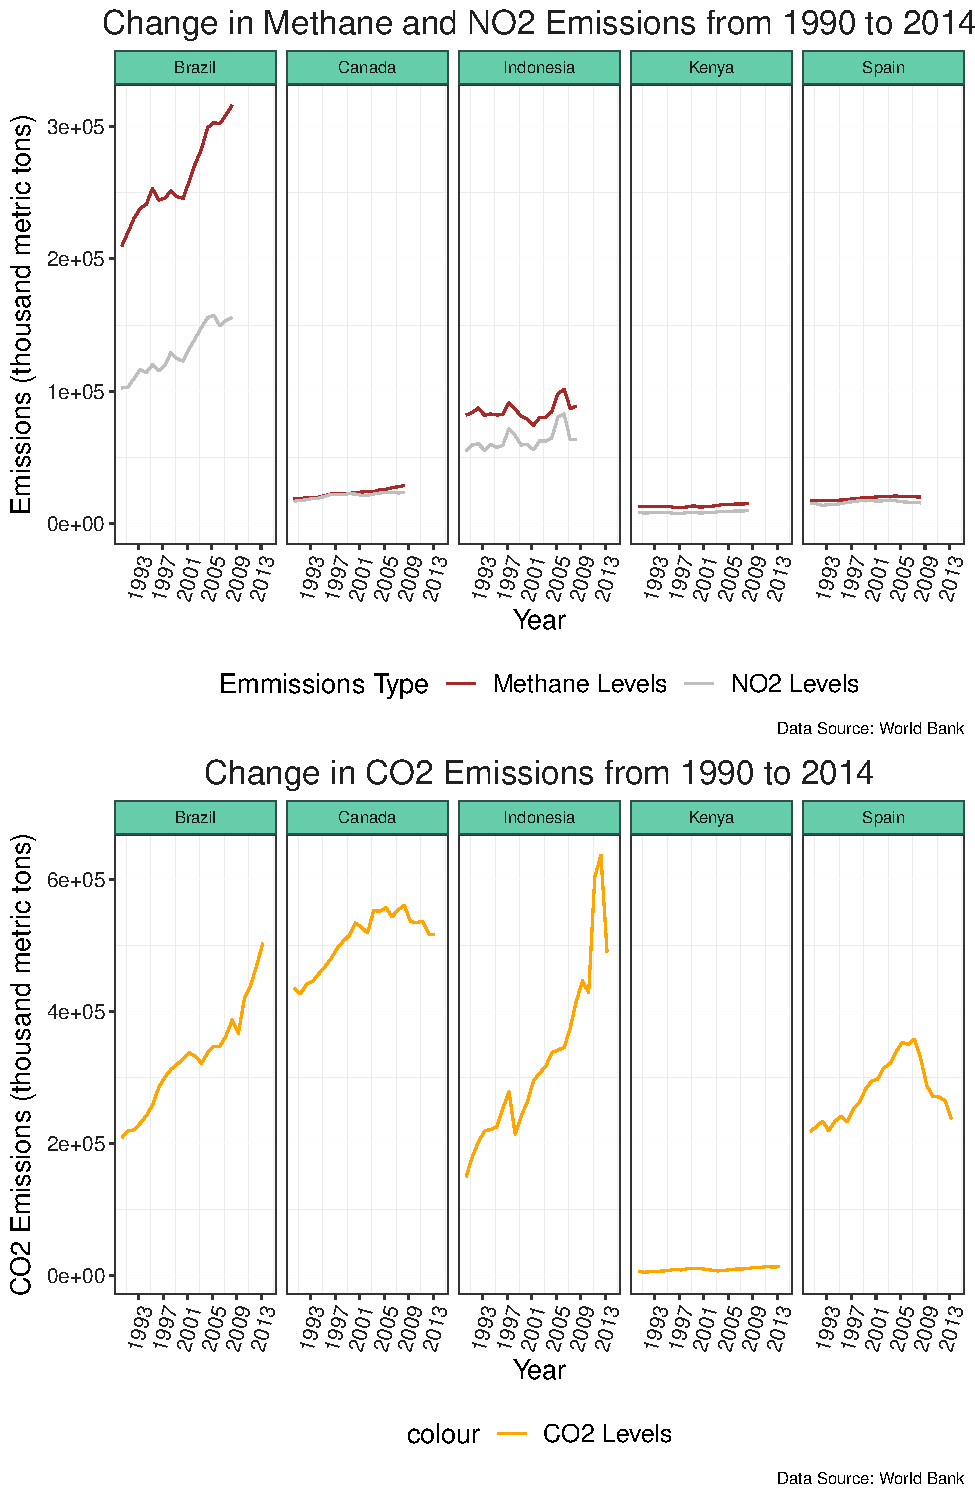
\includegraphics{Marx_ENV872_Project_files/figure-latex/unnamed-chunk-5-1.pdf}

\begin{verbatim}
## Warning: Removed 10791 rows containing missing values (geom_point).
\end{verbatim}

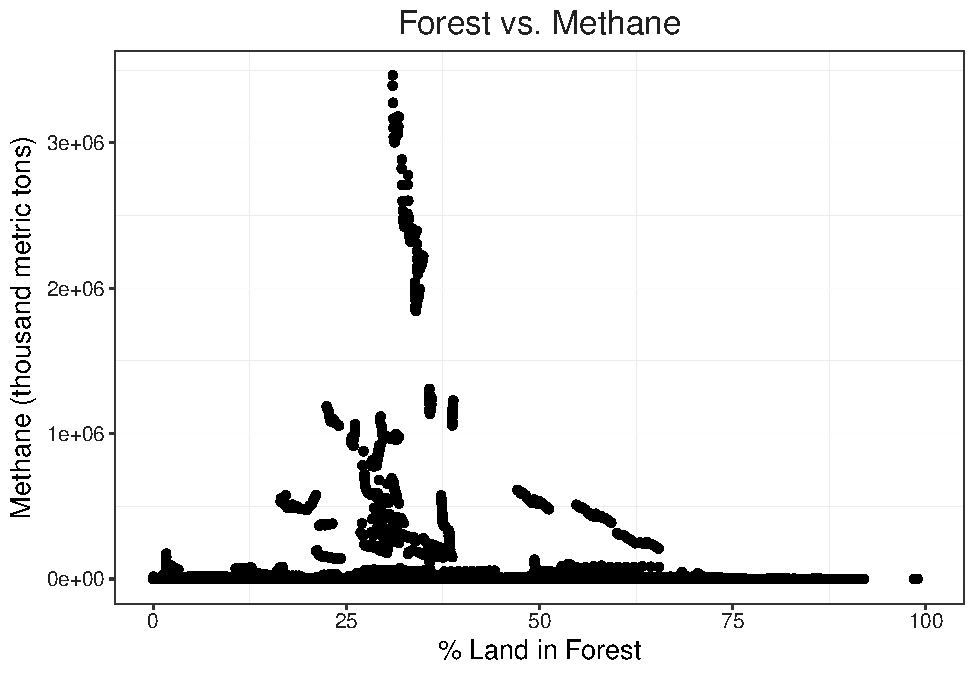
\includegraphics{Marx_ENV872_Project_files/figure-latex/unnamed-chunk-5-2.pdf}

\begin{verbatim}
## Warning: Removed 3900 rows containing missing values (geom_point).
\end{verbatim}

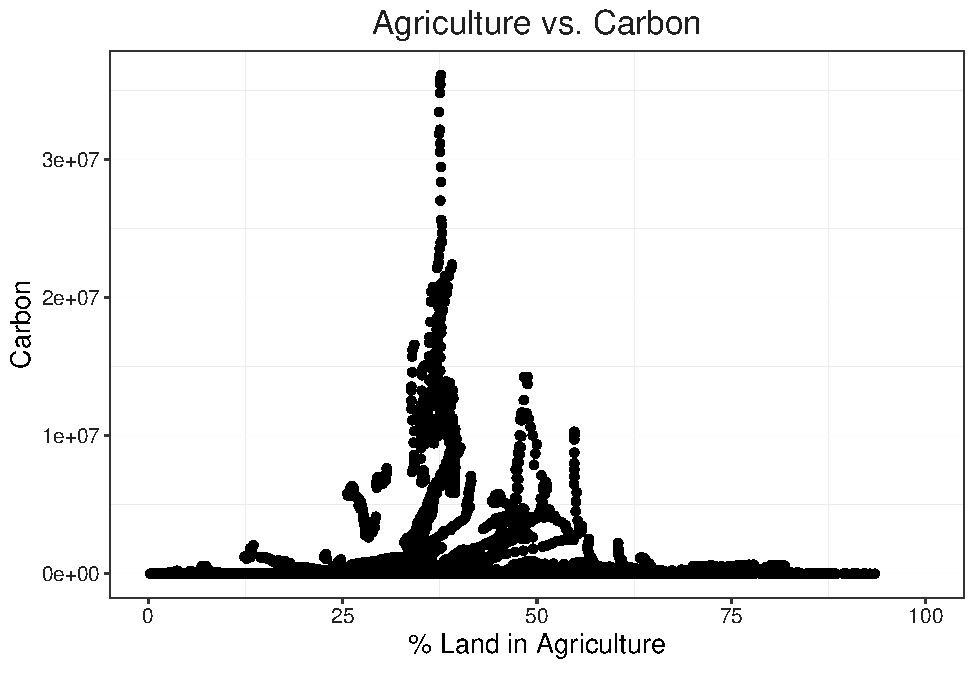
\includegraphics{Marx_ENV872_Project_files/figure-latex/unnamed-chunk-5-3.pdf}

\begin{verbatim}
## Warning: Removed 9616 rows containing missing values (geom_point).
\end{verbatim}

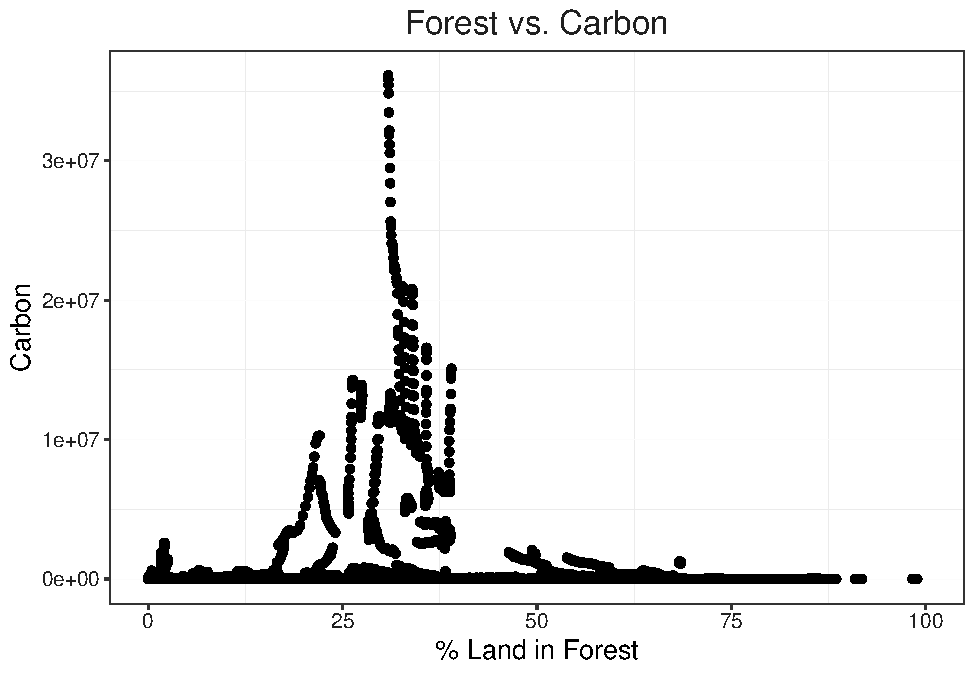
\includegraphics{Marx_ENV872_Project_files/figure-latex/unnamed-chunk-5-4.pdf}

\begin{verbatim}
## Warning: Removed 35 rows containing missing values (geom_path).

## Warning: Removed 35 rows containing missing values (geom_path).
\end{verbatim}

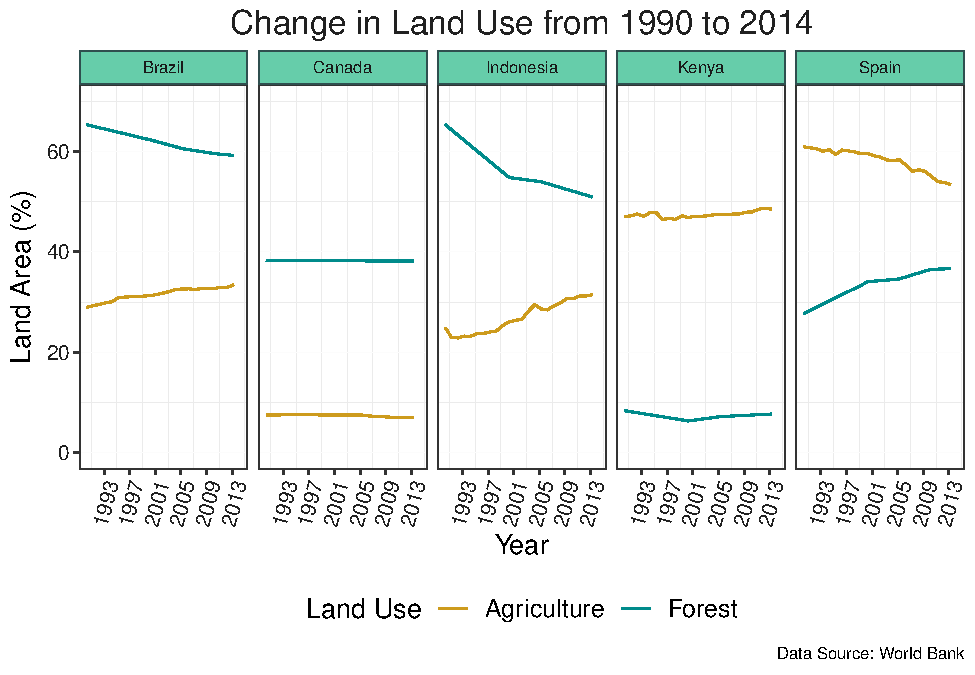
\includegraphics{Marx_ENV872_Project_files/figure-latex/unnamed-chunk-6-1.pdf}

\begin{verbatim}
## Warning: Removed 40 rows containing missing values (geom_path).

## Warning: Removed 40 rows containing missing values (geom_path).
\end{verbatim}

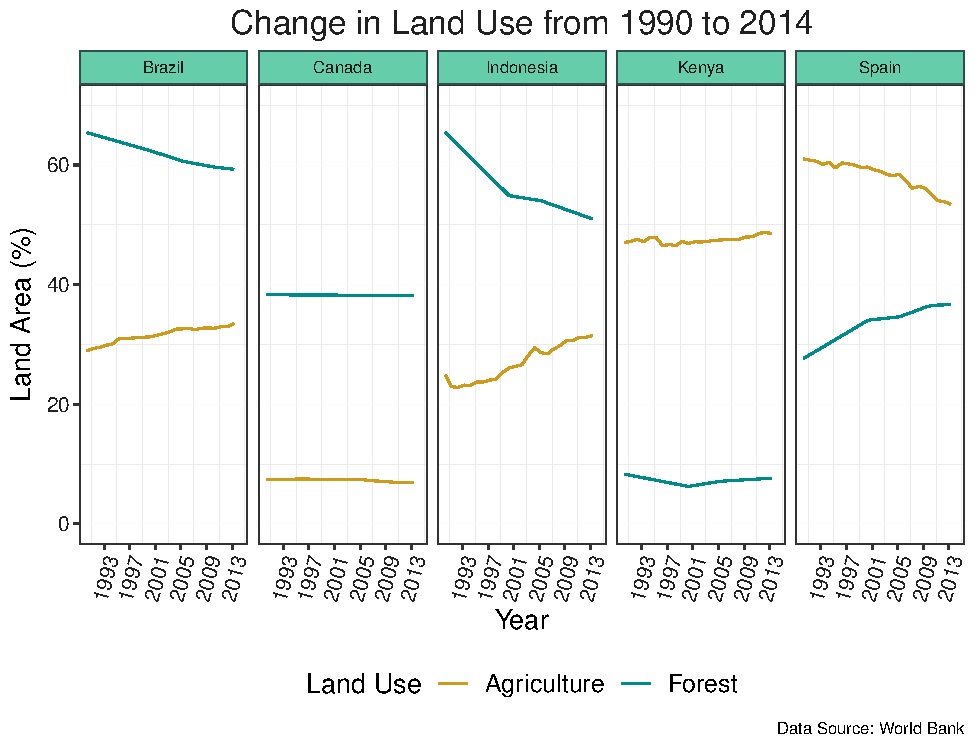
\includegraphics{Marx_ENV872_Project_files/figure-latex/unnamed-chunk-7-1.pdf}

\begin{verbatim}
\end{verbatim}

\begin{verbatim}
## Warning: Removed 35 rows containing missing values (geom_path).
\end{verbatim}

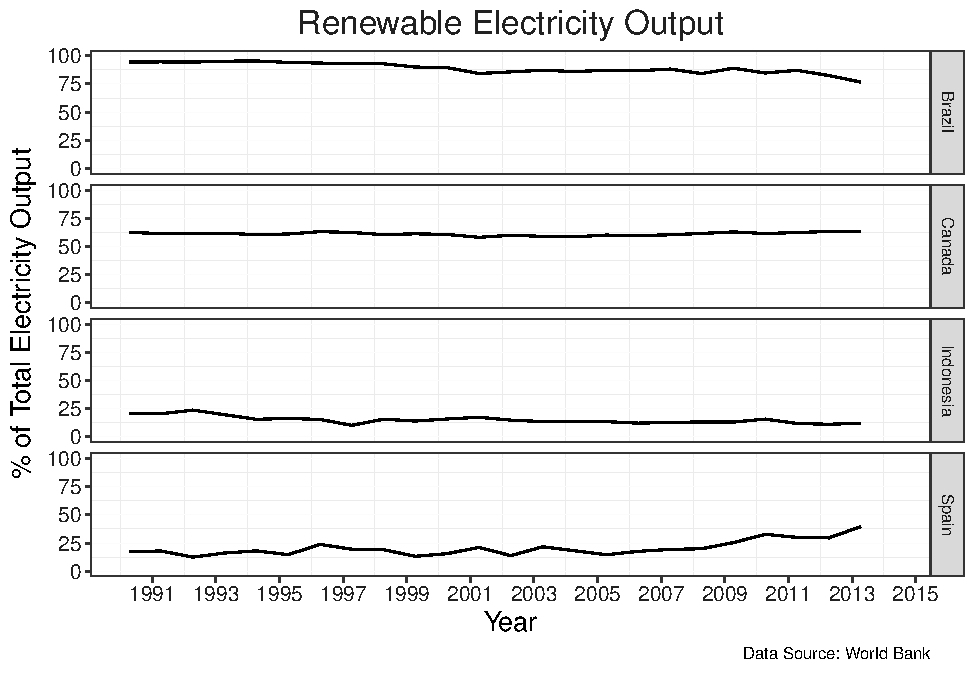
\includegraphics{Marx_ENV872_Project_files/figure-latex/unnamed-chunk-8-1.pdf}

\begin{verbatim}
## Warning: Removed 35 rows containing missing values (geom_path).

## Warning: Removed 35 rows containing missing values (geom_path).
\end{verbatim}

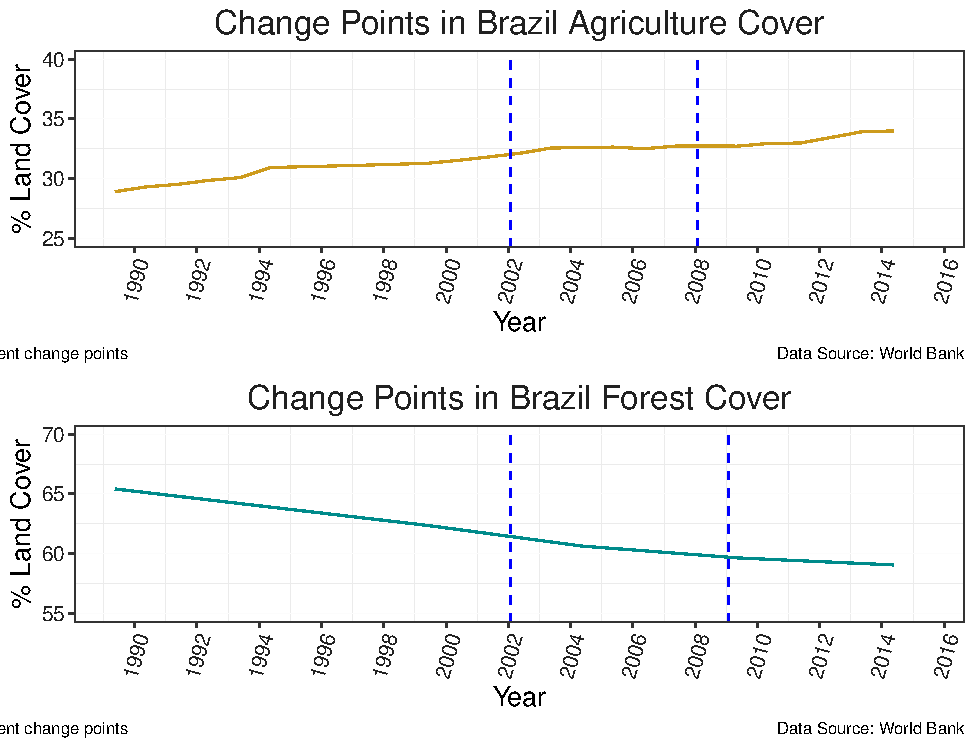
\includegraphics{Marx_ENV872_Project_files/figure-latex/unnamed-chunk-9-1.pdf}

\newpage

\section{Analysis}\label{analysis}

\begin{Shaded}
\begin{Highlighting}[]
\CommentTok{#Statistical Test 1: How has forest changed over time }
\NormalTok{Forest.Fixed <-}\StringTok{ }\KeywordTok{gls}\NormalTok{(}\DataTypeTok{data =}\NormalTok{ WB_Spread, }
\NormalTok{                    Forest }\OperatorTok{~}\StringTok{ }\NormalTok{Year,}
                    \DataTypeTok{method =} \StringTok{"REML"}\NormalTok{)}
\KeywordTok{summary}\NormalTok{(Forest.Fixed)}
\end{Highlighting}
\end{Shaded}

\begin{verbatim}
## Generalized least squares fit by REML
##   Model: Forest ~ Year 
##   Data: WB_Spread 
##        AIC     BIC    logLik
##   44741.09 44759.9 -22367.55
## 
## Coefficients:
##                Value Std.Error   t-value p-value
## (Intercept) 91.42949  6.525284 14.011572       0
## Year        -0.00485  0.000594 -8.156025       0
## 
##  Correlation: 
##      (Intr)
## Year -0.984
## 
## Standardized residuals:
##        Min         Q1        Med         Q3        Max 
## -0.7540709 -0.3205935 -0.1002986  0.1413443 15.6053463 
## 
## Residual standard error: 73.63104 
## Degrees of freedom: 3911 total; 3909 residual
\end{verbatim}

\begin{Shaded}
\begin{Highlighting}[]
\CommentTok{#Did not do "* Country)". Result shows on average Forest decreases by -.00485 each year. }
\end{Highlighting}
\end{Shaded}

A fixed effects model was used to see how land percetnage of forest area
accross the whoel data set changes over time. The results show that, on
average, forest decreases by -.00485\% each year.

\begin{Shaded}
\begin{Highlighting}[]
\NormalTok{Test1 <-}\StringTok{  }\KeywordTok{lme}\NormalTok{(}\DataTypeTok{data =}\NormalTok{ WB_Spread,}
\NormalTok{              Forest }\OperatorTok{~}\StringTok{ }\NormalTok{Year,}
              \DataTypeTok{random =} \OperatorTok{~}\DecValTok{1}\OperatorTok{|}\StringTok{ }\NormalTok{Country)}
\NormalTok{Test1}
\end{Highlighting}
\end{Shaded}

\begin{verbatim}
## Linear mixed-effects model fit by REML
##   Data: WB_Spread 
##   Log-restricted-likelihood: -22149.85
##   Fixed: Forest ~ Year 
##  (Intercept)         Year 
## 90.835100087 -0.004799758 
## 
## Random effects:
##  Formula: ~1 | Country
##         (Intercept) Residual
## StdDev:    30.78642 66.67633
## 
## Number of Observations: 3911
## Number of Groups: 223
\end{verbatim}

\begin{Shaded}
\begin{Highlighting}[]
\CommentTok{#On average forest decreases by -.0047% a year?}

\NormalTok{Forest.Fixed_Ag. <-}\StringTok{ }\KeywordTok{gls}\NormalTok{(}\DataTypeTok{data =}\NormalTok{ WB_Spread, }
\NormalTok{                    Forest }\OperatorTok{~}\StringTok{ }\NormalTok{Year }\OperatorTok{+}\StringTok{ }\NormalTok{Agriculture,}
                    \DataTypeTok{method =} \StringTok{"REML"}\NormalTok{)}
\NormalTok{Forest.Fixed_Ag. }\CommentTok{#-.5067}
\end{Highlighting}
\end{Shaded}

\begin{verbatim}
## Generalized least squares fit by REML
##   Model: Forest ~ Year + Agriculture 
##   Data: WB_Spread 
##   Log-restricted-likelihood: -22331.49
## 
## Coefficients:
##   (Intercept)          Year   Agriculture 
## 110.607315028  -0.004830877  -0.506739618 
## 
## Degrees of freedom: 3911 total; 3908 residual
## Residual standard error: 72.92833
\end{verbatim}

\begin{Shaded}
\begin{Highlighting}[]
\CommentTok{#Random effect??}
\NormalTok{Test2 <-}\StringTok{  }\KeywordTok{lme}\NormalTok{(}\DataTypeTok{data =}\NormalTok{ WB_Spread,}
\NormalTok{              Forest }\OperatorTok{~}\StringTok{ }\NormalTok{Year }\OperatorTok{+}\StringTok{ }\NormalTok{Agriculture, }
              \DataTypeTok{random =} \OperatorTok{~}\DecValTok{1}\OperatorTok{|}\StringTok{ }\NormalTok{Country)}
\NormalTok{Test2 }\CommentTok{# -.557}
\end{Highlighting}
\end{Shaded}

\begin{verbatim}
## Linear mixed-effects model fit by REML
##   Data: WB_Spread 
##   Log-restricted-likelihood: -22138.56
##   Fixed: Forest ~ Year + Agriculture 
##   (Intercept)          Year   Agriculture 
## 112.349788617  -0.004814667  -0.557561556 
## 
## Random effects:
##  Formula: ~1 | Country
##         (Intercept) Residual
## StdDev:    29.31384 66.60976
## 
## Number of Observations: 3911
## Number of Groups: 223
\end{verbatim}

\begin{Shaded}
\begin{Highlighting}[]
\KeywordTok{anova}\NormalTok{(Forest.Fixed, Test2) }\CommentTok{# Said: fitted objects with different fixed effects. REML comparisons are not meaningful.}
\end{Highlighting}
\end{Shaded}

\begin{verbatim}
## Warning in nlme::anova.lme(object = Forest.Fixed, Test2): fitted objects
## with different fixed effects. REML comparisons are not meaningful.
\end{verbatim}

\begin{verbatim}
##              Model df      AIC      BIC    logLik   Test  L.Ratio p-value
## Forest.Fixed     1  3 44741.09 44759.90 -22367.54                        
## Test2            2  5 44287.13 44318.48 -22138.56 1 vs 2 457.9608  <.0001
\end{verbatim}

\begin{Shaded}
\begin{Highlighting}[]
\CommentTok{#Add Electricity }
\NormalTok{Forest.Ag.Elec <-}\StringTok{ }\KeywordTok{gls}\NormalTok{(}\DataTypeTok{data =}\NormalTok{ WB_Spread, }
\NormalTok{                    Forest }\OperatorTok{~}\StringTok{ }\NormalTok{Year }\OperatorTok{+}\StringTok{ }\NormalTok{Agriculture }\OperatorTok{+}\StringTok{ }\NormalTok{ElectricityAccess,}
                    \DataTypeTok{method =} \StringTok{"REML"}\NormalTok{)}
\NormalTok{Forest.Ag.Elec}
\end{Highlighting}
\end{Shaded}

\begin{verbatim}
## Generalized least squares fit by REML
##   Model: Forest ~ Year + Agriculture + ElectricityAccess 
##   Data: WB_Spread 
##   Log-restricted-likelihood: -22287.92
## 
## Coefficients:
##       (Intercept)              Year       Agriculture ElectricityAccess 
##     129.772497937      -0.004179189      -0.560020533      -0.334328246 
## 
## Degrees of freedom: 3911 total; 3907 residual
## Residual standard error: 72.08392
\end{verbatim}

\begin{Shaded}
\begin{Highlighting}[]
\CommentTok{#Added electricity access to see whether a lack of electricity may contribute to deforestation from the use of biomass as an energy source. Electricity access appears to have a negative impact on forest (-.333) which may be because electricity is needed for some agricultural operations, or electricity is being produce via biofuels. }

\NormalTok{Forest.RE <-}\StringTok{ }\KeywordTok{gls}\NormalTok{(}\DataTypeTok{data =}\NormalTok{ WB_Spread, }
\NormalTok{                    Forest }\OperatorTok{~}\StringTok{ }\NormalTok{Year }\OperatorTok{+}\StringTok{ }\NormalTok{RenewableElectricity,}
                    \DataTypeTok{method =} \StringTok{"REML"}\NormalTok{)}
\NormalTok{Forest.RE}
\end{Highlighting}
\end{Shaded}

\begin{verbatim}
## Generalized least squares fit by REML
##   Model: Forest ~ Year + RenewableElectricity 
##   Data: WB_Spread 
##   Log-restricted-likelihood: -22357.42
## 
## Coefficients:
##          (Intercept)                 Year RenewableElectricity 
##         84.074720108         -0.004718623          0.181761849 
## 
## Degrees of freedom: 3911 total; 3908 residual
## Residual standard error: 73.40486
\end{verbatim}

\begin{Shaded}
\begin{Highlighting}[]
\CommentTok{#On that note, I was interested in whether there might be a relationship between forested land and renewable energy because energy produced from biomass is considered to be renewable. However, the result of my gls revealed that a 1 unit increase in renewable energy is associated with a .18% increase in forest land. }

\CommentTok{# Regression w/o time }
\NormalTok{Reg1 <-}\StringTok{ }\KeywordTok{lm}\NormalTok{(Forest }\OperatorTok{~}\StringTok{ }\NormalTok{Agriculture, WorldBank_Spread)}
\NormalTok{Reg1}
\end{Highlighting}
\end{Shaded}

\begin{verbatim}
## 
## Call:
## lm(formula = Forest ~ Agriculture, data = WorldBank_Spread)
## 
## Coefficients:
## (Intercept)  Agriculture  
##     52.5762      -0.4444
\end{verbatim}

\begin{Shaded}
\begin{Highlighting}[]
\CommentTok{#A 1 unit increas in agriculture leads to a -.44 decrease in forest }
\end{Highlighting}
\end{Shaded}

\begin{Shaded}
\begin{Highlighting}[]
\CommentTok{#Pettitts}
\CommentTok{#Statistical Test 2: Any change points for forest data?}
\KeywordTok{pettitt.test}\NormalTok{(WB_Spread}\OperatorTok{$}\NormalTok{Forest)}
\end{Highlighting}
\end{Shaded}

\begin{verbatim}
## 
##  Pettitt's test for single change-point detection
## 
## data:  WB_Spread$Forest
## U* = 458060, p-value = 1.459e-09
## alternative hypothesis: two.sided
## sample estimates:
## probable change point at time K 
##                            1428
\end{verbatim}

\begin{Shaded}
\begin{Highlighting}[]
\CommentTok{#Probable change point at time 1428 which doesn't exist.}

\KeywordTok{pettitt.test}\NormalTok{(WB_Brazil}\OperatorTok{$}\NormalTok{Forest)}
\end{Highlighting}
\end{Shaded}

\begin{verbatim}
## 
##  Pettitt's test for single change-point detection
## 
## data:  WB_Brazil$Forest
## U* = 90, p-value = 0.002386
## alternative hypothesis: two.sided
## sample estimates:
## probable change point at time K                            <NA> 
##                               9                              10
\end{verbatim}

\begin{Shaded}
\begin{Highlighting}[]
\CommentTok{#9}

\KeywordTok{pettitt.test}\NormalTok{(WB_Brazil}\OperatorTok{$}\NormalTok{Agriculture)}
\end{Highlighting}
\end{Shaded}

\begin{verbatim}
## 
##  Pettitt's test for single change-point detection
## 
## data:  WB_Brazil$Agriculture
## U* = 90, p-value = 0.002386
## alternative hypothesis: two.sided
## sample estimates:
## probable change point at time K                            <NA> 
##                               9                              10
\end{verbatim}

\begin{Shaded}
\begin{Highlighting}[]
\CommentTok{#9}
\end{Highlighting}
\end{Shaded}

Pettitt's applied to a single country (Brazil) initially detects a
change point in Forest and Agriculture in the same year.

\begin{Shaded}
\begin{Highlighting}[]
\CommentTok{#Statistical Test 3: Emmissions}

\NormalTok{AgMethane <-}\StringTok{ }\KeywordTok{gls}\NormalTok{(}\DataTypeTok{data =}\NormalTok{ WB_Spread,}
\NormalTok{                 Ag.Methane }\OperatorTok{~}\StringTok{ }\NormalTok{Year }\OperatorTok{+}\StringTok{ }\NormalTok{Agriculture,}
                 \DataTypeTok{method =} \StringTok{"REML"}\NormalTok{)}
\NormalTok{AgMethane }\CommentTok{#Ag. increases by 1, Ag Methane increases by 6.57}
\end{Highlighting}
\end{Shaded}

\begin{verbatim}
## Generalized least squares fit by REML
##   Model: Ag.Methane ~ Year + Agriculture 
##   Data: WB_Spread 
##   Log-restricted-likelihood: -56249.62
## 
## Coefficients:
##   (Intercept)          Year   Agriculture 
##  1.366512e+05 -5.517731e-01  6.577395e+02 
## 
## Degrees of freedom: 3911 total; 3908 residual
## Residual standard error: 428750.1
\end{verbatim}

\begin{Shaded}
\begin{Highlighting}[]
\NormalTok{ForestMethane <-}\StringTok{ }\KeywordTok{gls}\NormalTok{(}\DataTypeTok{data =}\NormalTok{ WB_Spread, }
\NormalTok{                  Ag.Methane }\OperatorTok{~}\StringTok{ }\NormalTok{Year }\OperatorTok{+}\StringTok{ }\NormalTok{Forest,}
                  \DataTypeTok{method =} \StringTok{"REML"}\NormalTok{)}
\NormalTok{ForestMethane }\CommentTok{#Forest increase by 1, methane increases by .035; Agricultural emmisions are not strongly related to deforestation. }
\end{Highlighting}
\end{Shaded}

\begin{verbatim}
## Generalized least squares fit by REML
##   Model: Ag.Methane ~ Year + Forest 
##   Data: WB_Spread 
##   Log-restricted-likelihood: -56245.46
## 
## Coefficients:
##  (Intercept)         Year       Forest 
## 1.289670e+05 1.195051e+00 3.563036e+02 
## 
## Degrees of freedom: 3911 total; 3908 residual
## Residual standard error: 428151.9
\end{verbatim}

\begin{Shaded}
\begin{Highlighting}[]
\NormalTok{Int.Methane <-}\StringTok{  }\KeywordTok{gls}\NormalTok{(}\DataTypeTok{data =}\NormalTok{ WB_Spread,}
\NormalTok{                    Ag.Methane }\OperatorTok{~}\StringTok{ }\NormalTok{Year }\OperatorTok{+}\StringTok{ }\NormalTok{Forest }\OperatorTok{*}\StringTok{ }\NormalTok{Agriculture,}
                    \DataTypeTok{method =} \StringTok{"REML"}\NormalTok{)}
\NormalTok{Int.Methane }\CommentTok{#Interaction of forest and agriculture: Increase of 1 leads to an increase of 98.856}
\end{Highlighting}
\end{Shaded}

\begin{verbatim}
## Generalized least squares fit by REML
##   Model: Ag.Methane ~ Year + Forest * Agriculture 
##   Data: WB_Spread 
##   Log-restricted-likelihood: -56201.69
## 
## Coefficients:
##        (Intercept)               Year             Forest 
##       217760.79850            1.76024        -3223.93002 
##        Agriculture Forest:Agriculture 
##        -2149.63528           98.85697 
## 
## Degrees of freedom: 3911 total; 3906 residual
## Residual standard error: 424598.6
\end{verbatim}

\begin{Shaded}
\begin{Highlighting}[]
\NormalTok{Forest.CO2 <-}\StringTok{ }\KeywordTok{gls}\NormalTok{(}\DataTypeTok{data =}\NormalTok{ WB_Spread, }
\NormalTok{                  CO2Emissions }\OperatorTok{~}\StringTok{ }\NormalTok{Year }\OperatorTok{+}\StringTok{ }\NormalTok{Forest,}
                  \DataTypeTok{method =} \StringTok{"REML"}\NormalTok{)}
\NormalTok{Forest.CO2 }\CommentTok{#1% increase in forest leads to a -235.25 decrease in CO2}
\end{Highlighting}
\end{Shaded}

\begin{verbatim}
## Generalized least squares fit by REML
##   Model: CO2Emissions ~ Year + Forest 
##   Data: WB_Spread 
##   Log-restricted-likelihood: -63931.14
## 
## Coefficients:
##  (Intercept)         Year       Forest 
## 420051.95130     56.36262   -235.25547 
## 
## Degrees of freedom: 3911 total; 3908 residual
## Residual standard error: 3059879
\end{verbatim}

\begin{Shaded}
\begin{Highlighting}[]
\NormalTok{Ag.CO2 <-}\StringTok{ }\KeywordTok{gls}\NormalTok{(}\DataTypeTok{data =}\NormalTok{ WB_Spread,}
\NormalTok{                 CO2Emissions }\OperatorTok{~}\StringTok{ }\NormalTok{Year }\OperatorTok{+}\StringTok{ }\NormalTok{Agriculture,}
                 \DataTypeTok{method =} \StringTok{"REML"}\NormalTok{)}
\NormalTok{Ag.CO2 }\CommentTok{# 1% increase in Ag. leads to an increase of 1493 kt of carbon. }
\end{Highlighting}
\end{Shaded}

\begin{verbatim}
## Generalized least squares fit by REML
##   Model: CO2Emissions ~ Year + Agriculture 
##   Data: WB_Spread 
##   Log-restricted-likelihood: -63929.71
## 
## Coefficients:
##  (Intercept)         Year  Agriculture 
## 342001.55481     57.45718   1493.99738 
## 
## Degrees of freedom: 3911 total; 3908 residual
## Residual standard error: 3059780
\end{verbatim}

\begin{Shaded}
\begin{Highlighting}[]
\NormalTok{Int.CO2 <-}\StringTok{ }\KeywordTok{gls}\NormalTok{(}\DataTypeTok{data =}\NormalTok{ WB_Spread,}
\NormalTok{                    CO2Emissions }\OperatorTok{~}\StringTok{ }\NormalTok{Year }\OperatorTok{+}\StringTok{ }\NormalTok{Forest }\OperatorTok{*}\StringTok{ }\NormalTok{Agriculture,}
                    \DataTypeTok{method =} \StringTok{"REML"}\NormalTok{)}
\NormalTok{Int.CO2 }\CommentTok{#How do you interperet this? }
\end{Highlighting}
\end{Shaded}

\begin{verbatim}
## Generalized least squares fit by REML
##   Model: CO2Emissions ~ Year + Forest * Agriculture 
##   Data: WB_Spread 
##   Log-restricted-likelihood: -63894.08
## 
## Coefficients:
##        (Intercept)               Year             Forest 
##      1130009.41628           59.26258       -22533.93863 
##        Agriculture Forest:Agriculture 
##       -17186.46246          611.63238 
## 
## Degrees of freedom: 3911 total; 3906 residual
## Residual standard error: 3042769
\end{verbatim}

\newpage

\section{Summary and Conclusions}\label{summary-and-conclusions}


\end{document}
